\documentclass[12pt, a4paper]{article}
\usepackage[utf8x]{inputenc}
\usepackage[spanish]{babel}
\usepackage{pdfpages}
\usepackage[T1]{fontenc} %Me deja combinar la negrita con las Mayusculas

\usepackage{amsmath}
\usepackage{amsfonts}
\usepackage{amssymb}
\usepackage{dsfont} %para el 1
\usepackage{mathrsfs}
\usepackage{enumitem} %Para la enumeracion con letras

\usepackage{graphicx} %para la imagen
\usepackage{subcaption} %para poner varias imagenes juntas
\usepackage{float}


\usepackage{chngcntr} %Para resetear el contador de las ecuaciones por secciones y subsecciones
\counterwithin*{equation}{section}
\counterwithin*{equation}{subsection}

\title{Tarea de Aprendizaje Estadístico}
\author{}
\date{}

\begin{document}
\begin{titlepage} %Inicio de la caratula del tp
	\centering
	  
\includegraphics[width=0.15\textwidth]{FIUBA_logo}\par
	  {\scshape\Large Universidad de Buenos Aires
      \\ Facultad de Ingenieria \par}
      {\scshape\small Año 2018 - 2er Cuatrimestre \par}
	  \vspace{1cm}
	  {\scshape\bfseries\LARGE Aprendizaje Estadístico, Teoría y aplicación\par}
	  \vspace{0.5cm}
	  \vspace{1cm}
      {\scshape\large Resúmen de la materia y devolutiva \par}
      \vspace{0.5cm
      \raggedright}
      \vspace{0.5cm}
    \centering
	  {\normalsize Sbruzzi, José Ignacio - Ingeniería Informática \#97452 \par}
      {\small  jose.sbru@gmail.com \par}
\end{titlepage} %Cerrado de la caratula del tp
\newpage
\tableofcontents
\newpage
\section{Clase 1 (31/8)}
La primera parte de esta clase fue un repaso de diversos temas que serán útiles durante la cursada:
\begin{itemize}
    \item Teorema de pitágoras
    \item espacios euclídeos
    \item Ortogonalidad
    \item Relación entre el producto interno y el coseno
    \item Desigualdad Cauchy-Schwartz
    \item Norma inducida
    \item Proyección Ortogonal
    \item Definición de esperanza
    \item El espacio algebraico de variables aleatorias
    \item Desigualdad de Markov
    \item Desigualdad de Chebyshev
    \item Desigualdad de Chernoff
    \item Desigualdad de Jensen
    \item Función convexa
    \item Esperanza condicional
\end{itemize}
La segunda parte de la clase se habló del problema de la comunicación digital para ilustrar la lógica por detrás de la construcción de un clasificador bayesiano.
Siendo $\delta(r)$ una función que predice el dígito (0 o 1) emitido a partir del recibido $r \in \{0,1\}$. $P(S=s|R=r)$ es la probabilidad de que se haya emitido el dígito $s$ dado que se recibió el dígito $r$.
$$\delta(r)=\mathds{1}\{\mathds{P}(S=1|R=r) > \mathds{P}(S=0|R=r)\}$$
Así, este clasificador toma la mejor decisión posible para la información que se tiene disponible ($r$), con lo cual es un clasificador bayesiano.

\section{Clase 2 (7/9)}
\subsection{Definiciones iniciales}
\subsubsection{Clasificador}
$$g:\mathds{R}^d\rightarrow\{ 1,2,...,M \}$$
$g(x)$ representa una conjetura respecto de la naturaleza de la distribución de las $x$. El clasificador se equivoca cuando $g(x) \neq y$.
\subsubsection{Calidad del clasificador}
Sea $(X,Y) \in \mathds{R}^d \times \{1,2, ..., M \}$ un par donde $X$ es una variable aleatoria que representa las propiedades observables y $Y$ la característica a predecir. Así, se define la pérdida de un clasificador como 
$L(g) = \mathds{P} ( g(X) \neq Y )$.
\subsubsection{Clasificador bayesiano}
Es el mejor clasificador, definido por
$$ argmin_{g:\mathds{R}^d \rightarrow \{1, ..., M\}}\{\mathds{P}( g(X) \neq Y )\} = g^{*}$$

$$L^{*}=L(g^{*})$$

No se da siempre que $L^{*}=0$ porque $Y$ podría no ser una función de $X$.

\subsubsection{Dataset de entrenamiento}
Se denota como $(X_i,Y_i), i = 1, 2, ..., n$; donde las parejas $(X_i,Y_i)$ son observaciones independientes e identicamente distribuidas, al igual que $(X,Y)$.

$$ D_n = \{(X_i,Y_i), i = 1, 2, ..., n\} $$

Así, en realidad, cuando aplicamos algoritmos de machine learning tenemos una g denotada como:
$$g(X,(X_1,Y_1), (X_2,Y_2), ..., (X_n,Y_n))$$
Donde $X$ es una nueva observación.

Es decir,
$$g_n:\mathds{R}^d \times ( \mathds{R}^d \times \{ 1, ..., M \})^n \rightarrow \{1,...,M\}$$

Así, tenemos $$L_n=L(g_n) = \mathds{P} ( g(X,(X_1,Y_1), ..., (X_n,Y_n)) \neq Y | (X_1,Y_1), ..., (X_n,Y_n))$$

Con lo cual $L_n$ es una variable aleatoria dependiente de las observaciones.
\subsection{Clasificador bayesiano para M=2}

Sean (con $A \subset \mathds{R}^d$, $x \in \mathds{R}^d$ , $y\in \{0,1\}$):

$$\mu(A)=\mathds{P}(x \in A)$$
$$\eta(x)=\mathds{P}(Y=1 | X=x)=\mathds{E}[Y|X=x]$$

Así, $$\eta(x)=\int_{C}\mathds{P}(Y=0|X=x) \mu(dx) + \int_{C}\mathds{P}(Y=1|X=x) \mu(dx)$$
Siendo $C=\mathds{R}^d \times \{0,1\}$.

Bajo estas condiciones, $$g^{*}(x)=\mathds{1}\{ \eta(x)>\frac{1}{2} \}$$

\section{Clase 3 (14/9)}

\subsection{Plug-in decision}

Una "plug-in decision" (decisión "enchufada") es una función $g$ definida por medio de una cierta función $\tilde{\eta}(x)$. Así, la función de decisión plug-in se define como:

$$g(x)=\mathds{1}\{ \tilde{\eta}(x) > \frac{1}{2}\}$$

En clase se demostró un teorema que establece que 

$$L(g) - L^{*}(g) \leq \int_{\mathds{R}^d} |\eta(x)-\tilde{\eta}(x)| \mu(dx) = 2 \mathds{E}[ \eta(X) - \tilde { \eta}(X) ]$$

Es decir, que si las funciones $\eta(x)$ y $\tilde{\eta}(x)$ son funciones similares (lo cual se ve más claramente en el miembro central de la fórmula anterior), los errores cometidos también serán similares. Es decir que, cuanto más se parezca $\eta$ a $\tilde{\eta}$, más cerca estará el error de $g$ del menor error posible (que es el de $g^{*}$).
\subsection{Convergencia debil y fuerte}
Una regla de clasificación $g_n$ es consistente si, para ciertas distribuciones de $(X,Y)$, se cumple:

$$\mathds{E}[L_n] = \mathds{P}(g_n(X,D_n)\neq Y) \rightarrow L^{*}\text{ cuando } n \rightarrow \infty$$

Y es fuertamente consistente si 

$$\mathop{lim}_{n \rightarrow \infty} L_n = L^{*} \text{ con probabilidad 1}$$

Una regla de clasificación es \textbf{universalmente consistente} si es fuertemente consistente para cualquier distribución de $(X,Y)$.

\subsection{Reglas basadas en particiones}
Muchas reglas de clasificación particionan el espacio en celdas disjuntas $A_i$, de forma que $$\mathds{R}^d = \mathop{\bigcup}_{i=1}^{\infty}A_i$$
La regla se basa en la "mayoría electoral", es decir, si $x$ pertenece a cierto $A_i$, entonces $g$ le asignará el valor más común de $y_i$ para los $x_i$ pertenecientes a $A_i$. Es decir,

$$g_n(x)=\mathds{1}\bigg \{ \mathop{\sum}_{i=1}^{n} \mathds{1}\{Y_i=1\} \mathds{1}\{X_i \in A(x)\} \geq \mathop{\sum}_{i=1}^{n} \mathds{1}\{Y_i=0\} \mathds{1}\{X_i \in A(x)\} \bigg \}$$

donde $A(x)$ es el $A_i$ al que pertenece $x$.
Sea el diámetro de un conjunto contenido en $\mathds{R}^d$ definido como:
$$diam(A)=\mathop{sup}_{x,y \in A} || x-y||$$

Y sea la cantidad de $X_i$ presentes en la misma celda que $x$ definida como:
$$N(x)=\mathop{\sum}_{i=1}^{n}\mathds{1}\{ X_i \in A(x) \}$$

La regla $g_n$ definida más arriba es consistente cuando se cumplen las siguientes condiciones:
$$diam(A(X))\rightarrow 0 \text{ en probabilidad}$$
$$N(X)\rightarrow \infty \text{ en probabilidad}$$

Es decir, los $A_i$ deben ser tales que su tamaño decrece a medida que crece $n$ pero la cantidad de puntos que contiene crece junto con $n$: deben ir reduciendo su tamaño pero no demasiado rápido, no deben tender a "vaciarse".

\subsection{La regla del histograma}
La regla del histograma es un caso especial de la regla de clasificación de la sección anterior en la que los $A_i$ son hipercubos de dimensión $d$ y de lado $h_n$.

Esta regla es universalmente consistente si se cumplen las siguientes condiciones:
$$h_n \rightarrow 0 \text{ cuando } n\rightarrow \infty$$
$$nh_n^d \rightarrow \infty \text{ cuando } n\rightarrow \infty$$

Estas condiciones son análogas a las de la sección anterior, con la diferencia de que cuando el espacio se parte en hipercubos se obtiene consistencia universal.

\section{Clase 4 (28/9)}
\subsection{El teorema de Stone}
El teorema de Stone indica condiciones bajo las cuales un clasificador que podría verse como una generalización de los de la clase 3 converge universalmente.

Se definen:
$$ \eta_n(x)=\mathop{\sum}_{i=1}^{n} \mathds{1}\{Y_i=1\} W_{ni}(x) $$
Siendo:
$$ \sum_{i=1}^n W_{ni}(x)=1 $$
Y se define la regla de clasificación como:
$$ g_n(x) = \mathds{1}\bigg \{ \sum_{i=1}^n \mathds{1}\{Y_i=1\} W_{ni}(x) \geq \mathds{1}\{Y_i=0\} W_{ni}(x) \bigg \} $$

$g_n$ converge universalmente cuando se cumplen las siguientes tres condiciones:

\subsubsection{Condición 1}
Existe una constante $c$ tal que, para cualquier función medible $f$ tal que $\mathds{E}[f(X)]<\infty$,
$$\mathds{E} \bigg \{ \sum_{i=1}^n W_{ni}(X)f(X_i) \bigg \} \leq c \mathds{E}[f(X)]$$

\subsubsection{Condición 2}
Para todo $a >0$,

$$\mathop{lim}_{ n \rightarrow \infty} \mathds{E} \bigg \{ \sum_{i=1}^n W_{ni}(X)\mathds{1}\{ || X_i -X ||>a \} \bigg \} = 0$$

\subsubsection{Condición 3}

$$ \mathop{lim}_{n \rightarrow \infty} \mathds{E} \bigg \{  \mathop{max}_{1 \leq i \leq n} W_{ni}(X)\bigg \} $$

\section{Clase 5 (5/10)}
\subsection{Desigualdad de Hoeffding}
Sean $X_1, ..., X_n$ variables aleatoreas independientes y sean $a_i$ y $b_i$ tales que $\mathds{P}(a_i \leq X_i \leq b_i)=1$, y sea $S_n=\sum_{i=1}^n X_i$. Entonces, para cualquier $\epsilon > 0$ se cumplen:
$$\mathds{P}(S_n - \mathds{E}[S_n] \geq \epsilon) \leq e^{-2 \epsilon^2 / \sum_{i=1}^n (b_i-a_i)^2}$$
y también
$$\mathds{P}(S_n - \mathds{E}[S_n] \leq - \epsilon) \leq e^{-2 \epsilon^2 / \sum_{i=1}^n (b_i-a_i)^2}$$

\subsection{Cómo estimar L}

Sea el estimador de $L$: $$\widehat{L}_{n,m}=\frac{1}{m} \sum_{j=1}^m \mathds{1} \bigg \{ g_n(X_{n+i}) \neq Y_{n+i} \bigg \}$$

$\widehat{L}_{n,m}$ es un estimador insesgado, es decir, $\mathds{E}[\widehat{L}_{n,m}|D_n]=L_n$

Aplicando la desigualdad de Hoeffding podemos deducir que:

$$ \mathds{P}(|\widehat{L}_{n,m}-L_n|>\epsilon | D_n) \leq 2e^{-2m\epsilon^2} $$

Es decir, independientemente de la distribución de $(X,Y)$ se puede acotar el error que tiene el estimador de $L_n$.
\subsection{Cómo elegir clasificadores}

$C$ es una família de funciones $\phi:\mathds(R)^d \rightarrow \{0,1\}$

$\phi^{*}_n$ es el clasificador de $C$ que minimiza la $L_n$ estimada: $$ \widehat{L_n}(\phi^{*}_n) \leq \widehat{L_n}(\phi) \text{ para todo } \phi \in C$$

Así, según descubierto por Vapnik y Chervonenkis:

$$L(\phi^{*}_n)-\mathop{inf}_{\phi \in C}L(\phi) \leq 2 \mathop{sup}_{\phi \in C} |\widehat{L_n}(\phi) - L(\phi)|$$

$$|\widehat{L_n}(\phi^{*}_n) - L(\phi^{*}_n)| \leq \mathop{sup}_{\phi \in C} |\widehat{L_n}(\phi) - L(\phi)|$$

Además, si $|C| \leq N$, tenemos que, para todo $\epsilon > 0$,

$$ \mathds{P} \bigg \{ \mathop{sup}_{\phi \in C} |\widehat{L_n}(\phi) - L(\phi)|>\epsilon \bigg \} \leq 2Ne^{-2n\epsilon^2} $$

Estos teoremas exhiben que utilizar el estimador de $L_n$ para elegir el $\phi$ dentro de una clase lleva a elegir funciones de decisión que minimizan $L$. Esto da fundamento teórico a los algoritmos de aprendizaje supervisado, en los cuales se utilizan métodos numéricos para buscar un $\phi$ que minimiza una estimación de la función de pérdida, la cual se calcula a partir de los datos de entrenamiento.
\section{Clase 6 (12/10)}
\subsection{Lema Borel-Cantelli}
Sea $A_n$ con $n=1,2,...$ una secuancia de ventos infinita.
Si se da que $$ \sum_{n=1}^{\infty} \mathds{P}(A_n) < \infty $$
Entonces: $$ \mathds{P}\big( \bigcap_{n=1}^{\infty} \bigcup_{m=n}^{\infty} A_m \big)=0 $$
\subsection{Teorema de Glivenko-Cantelli}
Sean $Z_1, ..., Z_n$ variables aleatorias identicamente distribuidas, con función de distribución $F$. Sea 
$$F_n(z)=\frac{1}{n} \sum_{i=1}^n \mathds{1} \{ Z_i \leq z \}$$
$$ \mathds{P} \bigg \{ \mathop{sup}_{z \in \mathds{R}} |F(z)-F_n(z)|>\epsilon \bigg \} \leq 8(n+1)e^{-n\epsilon^2/32}$$
Por el lema Borel-Cantelli:
$$ \mathop{lim}_{n \rightarrow \infty} \mathop{sup}_{z \in \mathds{R}} |F(z)-F_n(z)|=0 $$

La desigualdad de Vapnik-Chervonenkis puede comprenderse como una generalización de este teorema para cuando $z \in \mathds{R}^d$ (en este teorema se requiere $F$, lo cual implica que $z \in \mathds{R}$)

\subsection{Desigualdad Vapnik-Chervonenkis}
\subsubsection{Definiciones previas}
Sea $\mathds{A}$ un conjunto de conjuntos medibles. Sean $z_1, ...., z_n \in \mathds{R}^d$. Sea:
$$ N_{\mathds{A}}(z_1, ..., z_n)=\bigg | \big \{ \{ z_1, ..., z_n\} \cap A; \cap A \in \mathds{A} \big \} \bigg | $$

Sea entonces el N-avo coeficiente de destrozo/shattering/astillado de $\mathds{A}$:
$$ s(\mathds{A},n) = \mathop{max}_{(z_1,...,z_n) \in \{ \mathds{R}^d \}^n} N_{\mathds{A}}(z_1, ..., z_n)$$

$ s(\mathds{A},n)$ es la máxima cantidad de diferentes subconjuntos de n puntos que pueden ser ``pescados'' por la clase de conjuntos $\mathds{A}$. En cierta forma podría decirse que $ s(\mathds{A},n)$ es una medida de cuán ``versátil'', ``adaptable'' o ``expresiva'' $\mathds{A}$ es $\mathds{A}$.

Se definen Además

$$\nu(A)=\mathds{P}(Z_i \in A)$$
$$\nu_n(A)=\frac{1}{n} \sum_{i=1}^n \mathds{1} \{ Z_i \in A \}$$

Siendo $Z_i$ cualquier $Z_1, Z_2,... Z_n$ (son variables aleatorias en $ \mathds{R}^d $ identicamente distribuidas).

Entonces la desigualdad Vapnik-Chervonenkis indica que, para cualquier medida de probabilidad $\nu$, clase de conjuntos $\mathds{A}$, $n$ y $\epsilon>0$:

$$ \mathds{P} \big \{ \mathop{sup}_{A\in \mathds{A}} | \nu_n(A) - \nu(A) | > \epsilon \big \} \leq 8 s(\mathds{A},n)e^{-n\epsilon^2 / 32} $$

De esta desigualdad me llaman la atención dos cosas:
\begin{itemize}
  \item Fundamenta el fenómeno de "overfitting", ya que la distancia entre la estimación de $\nu$ y el $\nu$ real son más distantes cuando aumenta la capacidad expresiva de $\mathds{A}$
  \item Fundamenta el hecho de que el overfitting puede ser contrarrestado con más datos de entrenamiento, lo cual puede notarse en el hecho de que la cota decrece exponencialmente al crecer $n$.
\end{itemize}

\section{Clase 7 (19/10)}
En esta clase empezamos a ver regresión.
\subsection{Definiciones iniciales}
$$ m(x)=\mathds{E}[Y|X=x] $$
$$ m_n(x)=\sum_{i=1}^n W_{n,i}(x) Y_i $$
\subsection{Algunos criterios para medir la calidad de $m_n(x)$}
\subsubsection{Error de norma supremo}
$$ ||m_n - m||_{\infty} = \mathop{sup}_{x \in C} | m_n(x)-m(x)| \text{ con } C \in \mathds{R}^d $$
Mide el máximo error que comete $m_n$ en $C$, es decir, $m_n$ debe estar en un ``tubo'' que rodee a $m$.
\subsubsection{Error LP}
$$ ||m_n - m||_{p} = \int_{C} | m_n(x)-m(x)|^p dx $$
El error LP suma el error que comete $m_n$ a lo largo de todo $C$. Generalmente se usa $p=2$.
\subsection{4 paradigmas relacionados para estimar $m(x)$}
A continuación se presentan métodos que responden a la siguiente forma: $$ m_n(x)= \sum_{i=1}^n W_{n,i}(x) Y_i$$

Cada $W_{n,i}(x)$ representa el peso de $Y_i$ en el promedio ponderado.

Debe cumplirse que:

$$ \sum_{i=1}^n W_{n,i}(x) = 1 \text{ para todo $x$} $$
\subsubsection{Promedios locales}
Consiste en asignarle a $m_n(x)$ un valor que es el promedio de los $y_i$ que corresponden a los $k$ puntos $x_i$ más cercanos a $x$. Formalmente:

Sean los pares $(X_{(i)},Y_{(i)})$ una permutación de los datos de entrenamiento $D_n$ tal que $$ || x-X_{(1)} || \leq || x-X_{(2)} || \leq ... \leq || x - X_{(n)} || $$
Con esta permutación, se define $m_n$ como:
$$ m_n(x)= \frac{1}{k} \sum_{i=1}^k Y_{(i)}$$
Es decir que los pesos tienen los valores
$$ W_{n,i}=\frac{1}{k} \mathds{1} \big \{  \text{ $X_i$ es uno de los $k$ vecinos más cercanos a $x$} \big \}$$

Este método es una adaptación del algoritmo KNN para el caso de regresión.
\subsubsection{Estimador kernel de Nadaraya - Watson}
sea $K:\mathds{R}^d \rightarrow \mathds{R}^{+}$ un kernel.
Se definen los pesos para este caso:
$$ W_{n,i}(x)=\frac{ K \big ( \frac{x-X_i}{h} \big ) }{ \sum_{j=1}^n K \big ( \frac{x-X_j}{h} \big )} $$
Algunos kernels útiles son:
$$ K(x)=\mathds{1}\{ || x || \leq 1 \} $$
$$ K(x)=e^{-||x||^2}$$
Estos estimadores son una versión más interesante del caso anterior, ya que permiten establecer el peso de cada observación en función de su distancia a $x$, lo cual no hace el método anterior.

\subsubsection{Particiones}
Sea $\{A_{n,1}, A_{n,2}, ...\}$ una partición de $\mathds{R}^d$

$$ W_{n,i}(x) = \frac{\mathds{1}\{ X_i \in A_{n,i} \}}{ \sum_{j=1}^{n} \mathds{1}\{ X_j \in A_{n,i} \}} $$

Este método le asigna a los $x$ de una  misma partición el mismo valor, que es el promedio de los $Y_i$ correspondientes, es similar al método de promedios locales pero en este caso las particiones pueden ser independientes de $D_n$.

\subsubsection{Modelado local}

Según esta família de reglas, $g_n$ está definida con $l$ parámetros, es decir:

$$ g( \cdot , \{ a_k \}_{k=1}^{l} ):\mathds{R}^d \rightarrow \mathds{R} $$

Y los parámetros están elegidos de la siguiente forma:

$$ \{ a_k(x) \}_{k=1}^l = \mathop{argmin}_{\{b_k\}_{k=1}^l} \sum_{i=1}^n K\bigg (\frac{x-X_i}{h} \bigg ) \cdot \bigg ( Y_i - g \big (x, \{ b_k \}_{k=1}^{l} \big ) \bigg )$$

Así, se permite ``ajustar'' el promedio que genera el método Nadaraya-Watson por medio de una función con parámetros.

Así, $g_n$ podría pertenecer a una família de polinomios: $$ g_n(x,\{ a_k \}_{k=1}^l)=\sum _{k=1}^{l} a_k \cdot x^{k-1}$$

\subsubsection{Modelado global}

Se tiene una partición del espacio como en el método de particiones. El modelado globales una generalización del método de particiones.

Así, definimos:

$$ \mathds{F}_n = \Bigg \{ \sum_{j} a_j \mathds{1} \{ x \in A_{n,j}: a_j \in \mathds{R} \} \Bigg \} $$

$$ m_n = \mathop{argmin}_{f\in \mathds{F}_n} \Bigg \{ \frac{1}{n} \sum_{i=1}^n | f(X_i)-Y_i |^2 \Bigg \} $$

\subsubsection{Minimos cuadrados penalizados}

Se define un término de penalización $J_n(f)\geq 0$ que penaliza a $f$ según cuán violentamente cambia, permitiendo así elegir funciones $f$ que no hagan overfit sobre los datos de entrenamiento:

$$ m_n=\mathop{argmin}_f \Bigg \{ \frac{1}{n} \sum_{i=1}^n \big (f(X_i)-Y_i \big )^2 + J_n(f) \Bigg \} $$

Para el caso $d=1$, se utiliza como función de penalización $$ J_n(f)=\lambda_n \int |f^{(k)}(t)|^2 dt $$

Se puede generalizar $J_n$ a campos vectoriales, la fórmula utiliza derivadas parciales. El objetivo del término $J_n(f)$ es penalizar a las $f$ que tienen curvas violentas, lo cual es usual cuando se ajustan datos de entrenamiento a un polinomio.

\subsection{La maldición de la dimensionalidad}

La maldición de la dimensionalidad consiste en el hecho de que, cuantas más dimensiones tienen los datos, menos significativa es la distancia entre ellos. Así, si se tiene un hipercubo de dimensión $d$ con puntos distribuidos de forma uniforme sobre cada dimensión, la mayoría de los puntos se ubicarán sobre los bordes del cubo y estarán a una distancia muy similar los unos de los otros. Este efecto es cada vez más pronunciado a medida que crece $d$.

\subsection{Balance sesgo-varianza}

$$ \mathds{E} \Big \{ |m_n(x)-m(x)|^2 \Big \} = \mathds{E} \Big \{ | m_n(x) - \mathds{E} \big \{ m_n(x) \big \} |^2  \Big \} + \Big | \mathds{E} \big \{m_n(x) \big \} -m(x) \Big |^2$$

$$ \mathds{E} \Big \{ |m_n(x)-m(x)|^2 \Big \} = Var(m_n(x)) + |sesgo(m_n(x))|^2 $$

Así, $var$ es la varianza de la variable aleatoria $m_n(x)$, es decir, cuánto "le cree" a los datos: un algoritmo de machine learning con alta varianza es más propenso a sufrir overfitting. Una alta varianza de $m_n(x)$ implica que el modificar $D_n$ cambia $m_n(x)$ de forma significativa.

Por otro lado, el $sesgo$, cuantifica cuán "terco" es $m_n$. Un alto sesgo implica que incluso si la distribución de $D_n$ cambia, $m_n$ permanece similar. Esto está relacionado al fenómeno de underfitting.

El error de un $m_n$ es la suma de ambas componentes, ambas crecen en condiciones opuestas. 

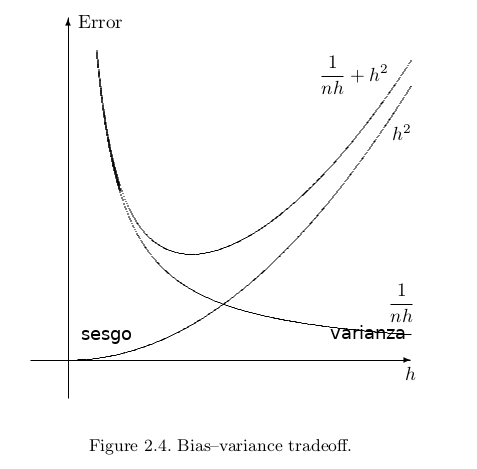
\includegraphics[scale=0.65]{bias-variance.png}

Ese gráfico está extraído de Gyorfi, muestra cómo se comportan el sesgo y la varianza al cambiar cuán detallado es un $g_n$ construído a partir de un kernel Nadaraya-Watson.

\subsection{Cómo comparar $g_n$ cuando no se dispone de las distribuciones}

\subsubsection{Método de resustitución}

En el método de resustitución se eligen los parámetros $p$ de manera de que la función de regresión $m_{n,p}(x)$ minimice

$$L(D_n) = \frac{1}{n} \sum_{i=1}^n | m_{n,p}(X_i)-Y_i |^2 $$

Esto lleva a resultados demasiado optimistas, ya que no es otra cosa que usar los mismos datos para entrenar el algoritmo y para medir cuán bueno es. Así, $g_n$ funcionará peor que lo esperado al predecir nuevos pares $(X,Y)$.

\subsubsection{Otro método de resustitución}

Se divide el conjunto de datos $D_n$ en $D_{n_1}$ y $D_{n_2}$ de forma que $D_n=D_{n_1} \cap D_{n_2}$. Luego se elige $p$ minimizando $L(D_{n_1})$ y se utiliza $g(\cdot,D_{n_2})$ para realizar predicciones.

\subsubsection{K-fold cross-validation (dividido de forma secuencial)}

Se definen $k$ conjuntos de pares $D_{n,k}$ de forma que $|D_{n,k}|=\frac{n}{k}$  y que $\bigcup_{l=1}^{k}D_{n,l}=D_n$.

Luego se eligen los parámetros $p$ minimizando

$$ \frac{1}{k} \sum_{l=1}^{k} \frac{1}{n/k} \sum_{i=\frac{n}{k}(l-1)+1}^{\frac{n}{k} l} | m_{n-\frac{n}{k},p}(X_i,D_{n,l} -Y_i) |^2 $$

Así, se tiene en cuenta el promedio de los errores de las $k$ particiones al mismo tiempo para obtener $p$.

\subsection{Clase 8 (26/10): Ley de los grandes números}

Sea $ f\in \mathds{F}_n$, y sea $f$ la función de regresión. Queremos minimizar el riesgo empírico $L_2$, es decir $$ \frac{1}{n} \sum_{i=1}^n |f(X_i)-Y_i|^2 $$

Se definen $Z=(X,Y)$, $Z_i=(X_i,Y_i)$, $i=1, ..., n$, $g_f(x,y)=|f(x)-y|^2$, $\mathds{G}_n=\{ g_f :f \in \mathds{F}_n\}$

El estimador del riesgo $L_2$ sólo es consistente sii $$ \mathop{sup}_{g\in\mathds{G}_n} \Bigg | \frac{1}{n} \sum_{i=1}^n g(Z_i) - \mathds{E}\{g(Z)\} \Bigg | \rightarrow 0 \text{ cuando } (n\rightarrow \infty) \text{ a.s. }$$

\subsection{Desigualdades exponenciales básicas}
Se cumple 

$$ \mathds{P} \Bigg \{ \mathop{sup}_{g \in \mathds{G}_n} \Bigg | \frac{1}{n} \sum_{j=1}^{n} g(Z_j)-\mathds{E}\{ g(Z) \} \Bigg | > \epsilon \Bigg \} \leq 2 | \mathds{G}_n| e^{-\frac{2n\epsilon^2}{B^2}} $$

Cuando $\mathds{G}_n$ es una clase finite y cumple
$$ \sum_{n=1}^{\infty} |\mathds{G}_n| e^{- \frac{2n\epsilon^2}{B^2}} < \infty$$

Para cualquier $\epsilon>0$

Cuando $\mathds{G}_n$ no es una clase finita, puede ser posible encontrar un $\mathds{G}_{n,\epsilon}$ finito que cumpla que todos los elementos de la família infinita están a una distancia supremo menor que $\epsilon$ que cualquier elemento de la família finita.

\subsection{Herramientas métricas}

Sea $d$ una distancia entre funciones.

Sean las bolas $B_{\epsilon}(g)=\{ g' \in g:d(g',g)<\epsilon \}$.

Un cubrimiento de $G$ es cualquier $G'=\{ g_1,..., g_N \}$ finito tal que $G' \subset G $ y $G \subset \bigcup_{i=1}^N B_{\epsilon}(g_i)$.


Sea el número de $\epsilon$ cubrimiento de $G$:
$$\mathds{N}(\epsilon,G,d)=\mathds{N}_d(\epsilon,G)=
\begin{cases}
 \infty & \text{si no existe ningún $\epsilon$ cubrimiento de $G$ con respecto a $d$} \\

 H & \text{en otro caso}\\
\end{cases}$$

$$H=\mathop{min}\{ n \text{ natural } : \text{ existe un $\epsilon$ cubrimiento de tamaño n de $G$ con respecto a d } \}$$

Cualquier colección finita $\{ g_1, g_2, ..., g_n\} \subset G$ tal que $d(g_i,g_j)\geq\epsilon\forall i\neq j$ es un $\epsilon$ empaquetado de $G$ con respecto a $d$.

Se define el número de $\epsilon$ empaquetado de $G$ con respecto a $d$ como $M(\epsilon,G,d)=M_d(\epsilon,G)$, que vale infinito para cualquier $n$ natural existe un $\epsilon$ empaquetado de $G$ de tamaño $n$. De lo contrario, vale

$$ \mathop{max}\big \{ n\in \text{ naturales }: \{ g_1, ..., g_n \} \text{ es un $\epsilon$-empaquetado de $G$ con respecto a $d$} \big \} $$

\subsection{Distancias posibles}
\subsubsection{Distancia supremo}
$$ d_{||\cdot||_{\infty}}(f,g)=\mathop{sup}_{z\in \mathds{R}^d}|f(z)-g(z)| $$
\subsubsection{Distancia LP}

$$ d_{L_p(\nu)}(f,g)=\bigg ( \int |f(z)|^p \nu(dz) \bigg )^{\frac{1}{p}}$$

\subsection{Lema}

Sea $n$ natural, y sea $G_n$ un conjunto de funciones $g:\mathds{R}^d \rightarrow [0,B]$ y $\epsilon > 0$. Entonces:

$$
\mathds{P}\Bigg \{ \mathop{sup}_{g\in \mathds{G}_n} \Big | \frac{1}{n} \sum_{j=1}^n g(Z_j)-\mathds{E}\{ g(Z) \} \Big | > \epsilon \Bigg \} \leq 2 \mathds{N}_{\infty} (\epsilon/3,\mathds{G}_n) e^{-\frac{2n\epsilon^2}{9B^2}}
$$

Además, si se cumple

$$
\sum_{n=1}^{\infty} \mathds{N}_{\infty} (\epsilon/3,\mathds{G}_n)e^{-\frac{2n\epsilon^2}{9B^2}}
$$

entonces también es se cumple

$$ \mathop{sup}_{g\in\mathds{G}_n} \Bigg | \frac{1}{n} \sum_{i=1}^n g(Z_i) - \mathds{E}\{g(Z)\} \Bigg | \rightarrow 0 \text{ cuando } (n\rightarrow \infty) \text{ a.s. }$$

Este lema indica que con una fam�lia $\mathds{G}_n$ discreta se pueden lograr funciones de regresión consrstentes

\section{Clase 8 (2/11)}
\subsection{Dimensi�n Vapnik-Chervonenkis}
escribir acá la definici�n(def9.6 pag144)
\subsection{Lema de Sawer}
copiar del cuaderno. Relaciona shatter coef"icient y vc dimension
Lo de downshift te lo regalo
Pag 148 teorema 9.4
La versi�n L1 y Lp del cuaderno
\section{Clase 9 (9/11)}




\end{document}
